\documentclass[a4paper]{article}
\usepackage{listings}
\usepackage{xcolor}
\usepackage {fontspec}
\usepackage {multicap}
\usepackage{fancyhdr}
\pagestyle{fancy}
\setromanfont{Lantinghei SC Extralight}
\setmonofont{Courier New}
\XeTeXlinebreaklocale ``zh''
\XeTeXlinebreakskip = 0pt plus 1pt
\textheight = 650pt
\lstset{
	%行号
   numbers=left,
  %背景框
   framexleftmargin=10mm,
   frame=none,
   %背景色
   %backgroundcolor=\color[rgb]{1,1,0.76},
   backgroundcolor=\color[RGB]{245,245,244},
   %样式
   keywordstyle=\bf\color{blue},
   identifierstyle=\bf,
   numberstyle=\tiny,
   numberstyle=\color[RGB]{0,192,192},
   commentstyle=\it\color[RGB]{0,96,96},
   stringstyle=\rmfamily\slshape\color[RGB]{128,0,0},
   %显示空格
   showstringspaces=false
 }

\begin{document}
<<<<<<< HEAD
\title{实验报告 实验九}
=======
\title{实验报告 实验八}
>>>>>>> 6bbb9151f7a29ac0f1c473835f4c5848087813a9
\author{姓名:王钦\quad 学号:13349112\quad 班级:计科二班}
\date{}

\maketitle
\section*{ 实验目的}
\hangindent=4em \hangafter=-10{
<<<<<<< HEAD
1. 学习FAT12文件系统组织方法,掌握其实现方法。\\
2. 利用FAT12文件系统实现原型操作系统的自身引导。\\
3. 扩展MyOS,利用FAT12文件系统实现加载用户程序。\\
}
\section*{ 实验内容}
\hangindent=4em \hangafter=-10{
  在实验五或更后的原型基础上,进化你的原型操作系统,原型保留原有特征的基础上,设计满足下列要求的新原型操作系统:\\
  (1)实现1.44MB软盘映像文件上的FAT12格式。\\
  (2)内核执行体以COM格式文件形式存放在映像的FAT12文件系统中,修改引导程序实现内核的加载.\\
  (3)将所有测试的用户程序放在在映像文件中的FAT12文件系统中,修改内核,实现从文件系统加载用户程序。\\
=======
1. 学习信号量机制的原理,掌握其实现方法。\\
2. 利用信号量机制,实现进程互斥和同步\\
3. 扩展MyOS,实现信号量机制\\
}
\section*{ 实验内容}
\hangindent=4em \hangafter=-10{
\indent 如果内核实现了信号量机制相关的系统调用,并在c库中封装相关的系统调用,那么,我们的c语言就也可以实现多进程同步的应用程序了。
例如:利用进程控制操作,父进程f创建二个子进程s和d,大儿子进程s反复向父进程f祝福,小儿子进程d反复向父进程送水果(每次一个苹果或其他水果),当二个子进程分别将一个祝福写到共享数据a和一个水果放进果盘后,父进程才去享受:从数组a收取出一个祝福和吃一个水果,如此反复进行。
参考程序如下:\\
{\scriptsize
	\begin{lstlisting}[language={C}]
Char fruit_disk;  苹果=1,雪梨=2,。。。
void main(){
	int s;
	s=GetSem(0);
	if (fork())
		while(1) { p(s); p(s); myprintf(words);fruit_disk=0;}
	else
		if(fork())
		while(1) {
		putwords(“Father will live one year after anther for ever!”);
		v(s)
		}else
		while(1) { putfruit(); v(s)}
}
Void putwords(char *w) {  将祝福一个词一个词放进words[];}
Void putfruit() {    随机选择一个水果放进fruit_disk; }
如果顺利,编译连接这个用户程序,产生一个com文件,放进程原型操作系统映像盘中,试试有何结果?

\end{lstlisting}}
>>>>>>> 6bbb9151f7a29ac0f1c473835f4c5848087813a9
}

\section*{ 实验平台}
\hangindent=4em \hangafter=-10{
  xxd+dd+gcc+ld+nasm+Linux+vim\\
  实验报告编辑:Latex
}

\section*{ 算法流程图}
\hangindent=4em \hangafter=-10{
<<<<<<< HEAD
  \begin{center} 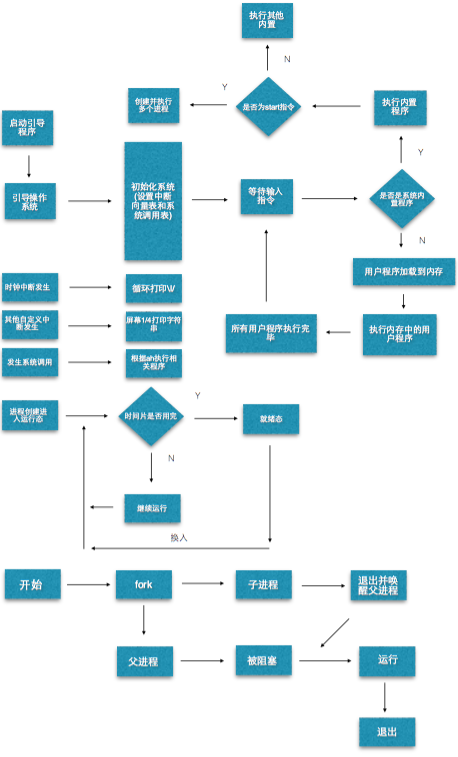
\includegraphics[scale=0.5]{Illustrations/flow0.png} \mfcaption{other}\end{center}
  \begin{center} 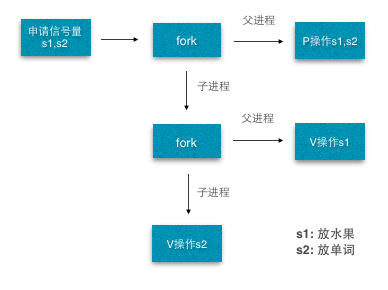
\includegraphics[scale=0.5]{Illustrations/flow1.png} \mfcaption{process}\end{center}
=======
  \begin{center} 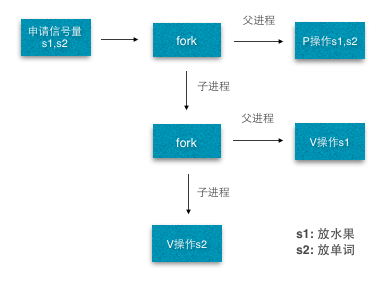
\includegraphics[scale=0.5]{Illustrations/flow.png} \mfcaption{flow}\end{center}
>>>>>>> 6bbb9151f7a29ac0f1c473835f4c5848087813a9
}

\section*{ 功能一览}
\hangindent=4em \hangafter=-50{
	{\large 1. 系统内置功能:}\\
		\indent \verb| terminal|,装载内核shell,为用户提供一个与操作系统交互的工具,开机后自动进入,以下所有功能都在terminal中交互\\
		\indent \verb| clear|, 清除当前屏幕所有字符,刷新屏幕\\
		\indent \verb| help|, 显示系统帮助信息\\
		\indent \verb| python |, python 扩展,类似python命令行工具,可以使用这个工具输入计算表达式返回计算结果,目前只支持加法减法\\
		\indent \verb| start|, 开始创建并执行四个进程并且每秒18.2次的调度,分别在屏幕\verb|1/4|处打印一些个性化信息( 不同配置的虚拟机动画速度不一样,建议使用bochs测试)\\\\
	{\large 2. 用户程序:}\\
		\indent \verb| run |,软盘中含有两个用户程序,输入\verb|run 12|,可分别执行两个用户程序,当然也可以通过改变执行序列来改变执行的顺序\\\\
	{\large 3. 自定义中断:}\\
		\indent 时钟中断:通过PTR每秒发出18.2次的信号来从8592芯片的RT0引脚发出终端号\verb|int 08h|来触发的用户时钟软中断\verb| int 1ch|,实现在\verb|terminal|的右下角
	  一个横杠在转动.\\
		\indent 另外有自定义中断\verb|int 33h,int 34h,int 35h,int 36h|分别在屏幕四分之一的位置打印个性化信息\\\\
	{\large 4. 进程调度:}\\
		\indent 软盘中共存放了用于展示进程调度的六个应用程序,其中一个应用程序为监听用户键盘事件然后退出多进程调度状态回到\verb| terminal|每个应用程序分别代表一个进程。开启装载进程并进行进程调度由\verb|1|中系统内置功能的\verb| start|指令激活。\\
		\\
	{\large 5. 进程\verb|fork,wait,exit|:}\\
		\indent 具体使用在第六个进程中,执行\verb|start|后即可看到包括第六个进程在内全部进程执行的结果。\\\\
	{\large 6. 使用信号量解决进程间的同步:}\\
<<<<<<< HEAD
		\indent 具体使用在第六个进程中,执行\verb|start|后即可看到包括第六个进程在内全部进程执行的结果。\\\\
	{\large 7. 文件系统}\\
		\indent 硬盘内容的加载均使用unix文件系统的形式管理,执行\verb|ls| 命令可以查看用户区有哪些文件\\\\
=======
		\indent 具体使用在第六个进程中,执行\verb|start|后即可看到包括第六个进程在内全部进程执行的结果。
>>>>>>> 6bbb9151f7a29ac0f1c473835f4c5848087813a9
}

\section*{ 实验步骤及效果图}
\hangindent=4em \hangafter=-50{
	\begin{enumerate}
<<<<<<< HEAD
		\item 运行\verb| ls|命令,查看所有用户程序文件
		\begin{center} 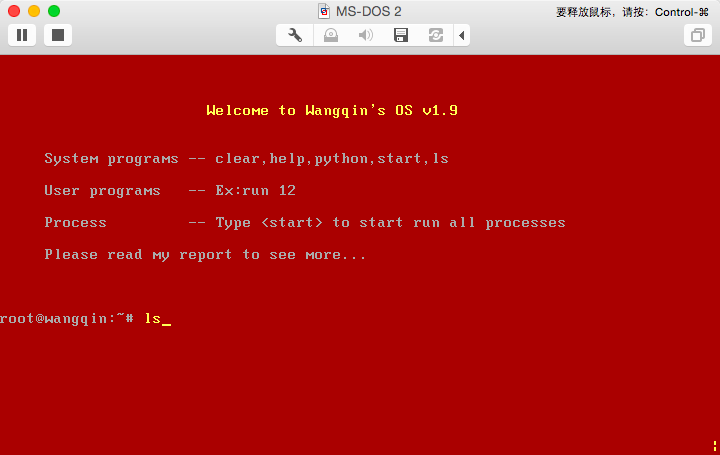
\includegraphics[scale=0.4]{Illustrations/ls.png} \mfcaption{ls}\end{center}
		\begin{center} 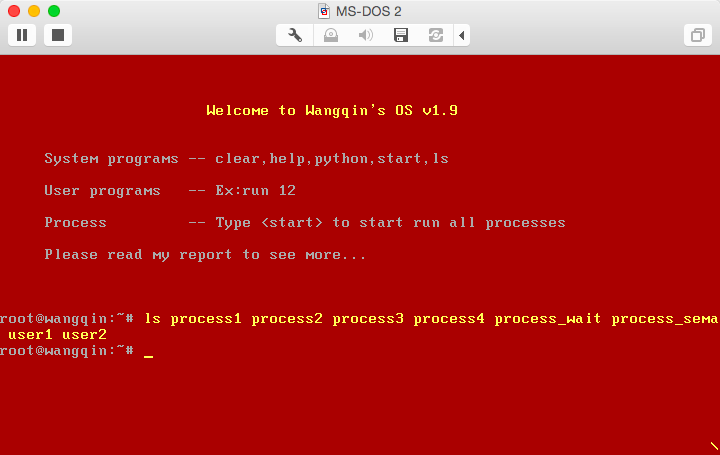
\includegraphics[scale=0.4]{Illustrations/ls_resu.png} \mfcaption{ls\_result}\end{center}
		\item 运行\verb| run user1|命令,运行第一个用户程序
		\begin{center} 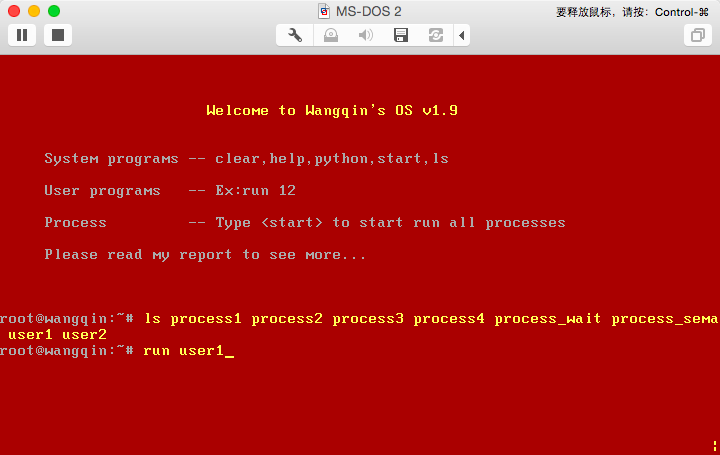
\includegraphics[scale=0.4]{Illustrations/run.png} \mfcaption{run}\end{center}
		\begin{center} 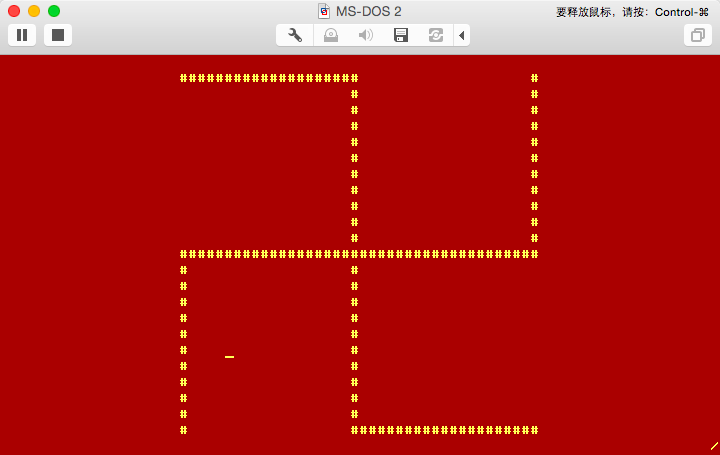
\includegraphics[scale=0.4]{Illustrations/run_resu.png} \mfcaption{run\_result}\end{center}
=======
		\item 运行\verb| start|命令,开始执行并调度所有进程
		\begin{center} 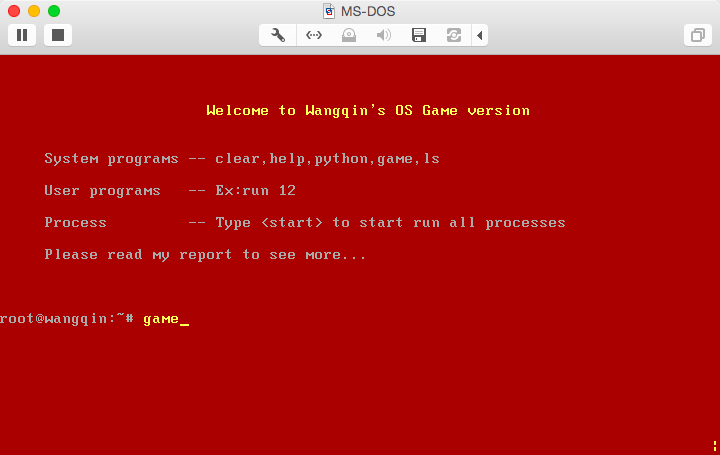
\includegraphics[scale=0.4]{Illustrations/start.png} \mfcaption{start}\end{center}
		\item 下图为执行画面,利用信号量实现了进程间的同步关系,儿子放水果的时候随机放1或2(1代表苹果,2代表雪梨)可以看到每次都是两个儿子进程putfruit,putwords
		  之后再让第一个进程执行打印出句子和水果。
		\begin{center} 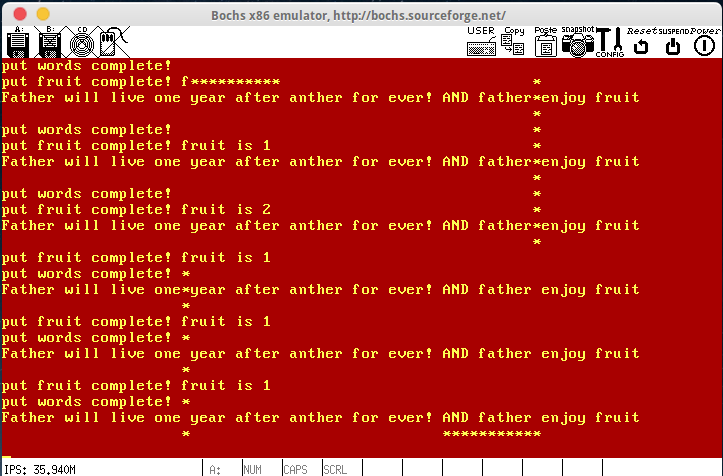
\includegraphics[scale=0.4]{Illustrations/semaphore.png} \mfcaption{start}\end{center}
>>>>>>> 6bbb9151f7a29ac0f1c473835f4c5848087813a9
	\end{enumerate}
}
\section*{ 内存和软盘存储管理}
\hangindent=4em \hangafter=-50{
1. 引导程序加载到内存0x7c00处运行\\
2. 引导程序将操作系统加载到0x7e00处运行\\
3. 操作系统讲用户程序加载到0x1000处运行\\
4. 软盘第0个柱面的第一个扇区存储操作系统引导程序\\
5. 软盘第0个柱面剩下所有扇区2~36扇区存储操作系统内核\\
6. 软盘第\verb|1,2,3,4,5,6|柱面分别存储六个进程代码\\
7. 软盘第\verb|7,8|柱面分别存储两个用户程序的程序代码\\\\
{\large 栈结构}\\
	\indent 内核栈:从内存的\verb| 0xffff|开始向下扩展\\
	\indent 用户栈:从内存的\verb| 0x1000|开始向下扩展\\
	\indent 进程栈:第i个进程对应的进程栈从内存的\verb| i*0x800|开始向下扩展\\
	\indent 第六个进程之后会有点特殊每次进程栈会加0x1000(主要为了保障fork后的进程有足够大的栈),例如第六个是0x3000,
	第七个是0x4000,第八个是0x5000...\\\\
更多细节信息请阅读我的Makefile文件
}
\section*{ 系统目录结构}
\hangindent=4em \hangafter=-50{
{\scriptsize
  \setmonofont{Lantinghei SC Extralight}
\begin{verbatim}
.
├── Makefile							makefile 文件
├── README
├── bochsrc                             bochs配置文件
├── boot.asm                            引导程序
├── disk.img							镜像文件
├── kernel                              目录中存放内核相关代码
<<<<<<< HEAD
│   ├── fcb.h							文件控制模块
=======
>>>>>>> 6bbb9151f7a29ac0f1c473835f4c5848087813a9
│   ├── os.asm                           主要为os.c提供函数实现.
│   ├── os.c                            为内核主要控制模块
│   ├── os.h                            主要为os.c提供函数实现.
│   ├── os_syscall.asm                  系统调用相关代码
│   ├── osclib.c                        为osclib.c提供更底层的函数封装
│   ├── oslib.asm                       初始化系统调用和设置系统调用相关模块
│   ├── pcb.h							进程控制模块
│   ├── process.c                       进程调度创建以及信号量相关代码
│   ├── terminal.c                      装载shell的工具
│   └── terminal.h
├── muti_process.h                      fork,wait,wakeup,printf等声明实现
├── osclib_share.c                      内核和用户的共享库(使用户程序体积减少)。
├── oslib_share.asm                     内核和用户的共享库(使用户程序体积减少)。
├── process1.asm                        第一个进程
├── process2.asm                        第二个进程
├── process3.asm                        ..
├── process4.asm                        ..
<<<<<<< HEAD
├── process_semaphore.c                 father's gifts 进程(信号量解决)
=======
├── process_semaphore.c                 father's gifts 进程(信号量解决)<本次实验要求>
>>>>>>> 6bbb9151f7a29ac0f1c473835f4c5848087813a9
├── process_wait_key.asm                监听退出进程
├── python_extension.c                  Python扩展
├── report                              实验报告目录
│   ├── Illustrations                   插图
│   │   └── flow.png
│   └── report.tex						Latex文件
├── snapshot.txt
├── usr1.asm							用户程序1
├── usr2.asm							\ldots
└── usrlib.asm							用户程序专用汇编库(不与内核共享)

3 directories, 31 files
\end{verbatim}}
}

\setmonofont{Courier New}

\section*{ 主要函数模块}
\hangindent=4em \hangafter=-50{
	\begin{enumerate}
<<<<<<< HEAD
\item \verb|fcb|,文件控制模块,记录着文件的属性和一些信息的一组数据,\verb|name|文件名,\verb|f_num|文件编号,\verb|f_size|文件大小,\verb|f_addr|文件地址,\verb|f_toMem|文件加载到内存的地址.
{\scriptsize\begin{lstlisting}[language={C}]
struct fcb{
 const char *name;
 char f_num;
 char f_size;
 char f_addr;		//block num
 int f_toMem;		//
};
struct fcb FCB_array[ file_sum];
 		\end{lstlisting}}
	\item \verb|loadfile|,将文件加载到指定内存地址
{\scriptsize\begin{lstlisting}[language={C}]
	load_user:
	;load os to mem

	mov ax,cs
	mov es,ax

	mov cx,1;

	;next_lu:


	mov dx,bp	;backup
	mov bp,sp
	mov ch,[ bp+4]		; 柱面/磁道  every zhumian  has one user program 37~72  73~108 109~144		ch = 7~8 is user
	mov bx,[ bp+8] ;add to 0x100 mem
	
	mov bp,dx

	mov dl,0		; 软盘
	mov dh,0		; 磁头:正面

	xor ax,ax
	mov es,ax ;made es zero,ex:bx is addr of mem 
	mov ax,0215h	;count 

	int 13h
	;cmp ch,6
	;je sixun
	;jmp nextaa
	;sixun:
	;jmp $
	;nextaa:

ret

\end{lstlisting}}
\item 一些变量说明
{\scriptsize\begin{lstlisting}[language={C}]

BaseOfLoader			equ	1000h	    ; 根目录 被加载到的位置 ----  段地址
OffsetOfLoader	        equ	4000h	    ; 根目录 被加载到的位置 ---- 偏移地址
RootDirSectors	        equ	14		    ; 根目录占用的扇区数
SectorNoOfRootDirectory	equ	19	        ; 根目录区的首扇区号
SectorNoOfFAT1	        equ	1		    ; FAT#1的首扇区号 = BPB_RsvdSecCnt
DeltaSectorNo		    equ	17		    ; DeltaSectorNo = BPB_RsvdSecCnt + 
; (BPB_NumFATs * FATSz) - 2 = 1 + (2*9) -2 = 17
; 文件的开始扇区号 = 目录条目中的开始扇区号 
; + 根目录占用扇区数目 + DeltaSectorNo

wRootDirSizeForLoop	    dw	RootDirSectors	; 根目录区剩余扇区数
; 初始化为14,在循环中会递减至零
wSectorNo				dw	0           ; 当前扇区号,初始化为0,在循环中会递增
bOdd					db	0			; 奇数还是偶数FAT项
filename                dw  0           ; 文件名指针
baseAddress             dw  0           ; 文件加载段地址
offsetAddress           dw  0           ; 文件加载偏移地址

BPB_BytsPerSec			dw 512          ; 每扇区字节数
BPB_SecPerTrk	        dw 18	        ; 每磁道扇区数
BS_DrvNum		        db 0	        ; 中断 13 的驱动器号(软盘
\end{lstlisting}}
=======
	\item \verb|pcb.h: semaphore|,定义信号量结构体,\verb|block_queue|为阻塞队列,head,tail分别为阻塞的队列的头部和尾部,count表示
	信号量的值,used表示是否正在被使用。
		{\scriptsize\begin{lstlisting}[language={C}]
			struct semaphore{
				int count;
				int block_queue[ process_num_MAX+1];
				int used;
				int head;
				int tail;
			};
 		\end{lstlisting}}
	\item \verb|muti_process.h: GetSem|09号系统调用获取信号量.
		{\scriptsize\begin{lstlisting}[language={C}]
		char GetSem( char value ){
			__asm__("cli");
			__asm__("mov $9,%ah");
			__asm__("int $0x80");
			__asm__("pop %ebx");
			__asm__("pop %ebx");
			__asm__("pop %bx");
			__asm__("sti");
			__asm__("jmp *%bx");
		}
 		\end{lstlisting}}
	\item \verb|process.c: do_getsem|,获取信号量,同时标志此信号量已被使用,返回信号量的主键,未找到可用的返回-1
		{\scriptsize\begin{lstlisting}[language={C}]
		void do_getsem(){
			if_find = 0;
			for(i=0;i<=sema_num_MAX;i++){
				if( sema_array[ i].used == 0){
					sema_array[ i].used = 1;
					if_find = 1;
					sema_index = i;
					break;
				}
			}
			if( !if_find){
				return_sema(-1);
			}
			return_sema( sema_index);
			__asm__("pop %cx");
			__asm__("pop %ecx");

			__asm__("pop %bx");
			__asm__("pop %bx");
			__asm__("pop %bx");
			__asm__("jmp *%bx");  //back to os_syscall callrun
		}
 		\end{lstlisting}}
	 \item \verb|muti_process.h: sema_P|,使用10号系统调用,stosi函数将信号量暂存在si寄存器中中断时传递给内核.
		{\scriptsize\begin{lstlisting}[language={C}]
				void sema_P( int s){
					__asm__("cli");
					stosi( s);
					__asm__("pop %cx");
					__asm__("mov $10,%ah");
					__asm__("int $0x80");
					__asm__("pop %ebx");
					__asm__("pop %ebx");
					__asm__("pop %bx");
					__asm__("sti");
					__asm__("int $0x1c");
					__asm__("jmp *%bx");
				}
 		\end{lstlisting}}
	 \item \verb|process.c: do_P|,执行对信号量的P操作,如果发现信号量小于0则阻塞当前进程。sitoindex()函数将之前保存在si中
	的信号量拷贝到\verb|s_index|中,使用\verb|s_index|即可定位到对应的semaphore.阻塞队列使用循环队列的方式控制。\verb|w_is_r|为当前正在运行的进程
	{\scriptsize\begin{lstlisting}[language={C}]
	void semaBlock( char s){
		PCB_queue[ w_is_r].process_status = BLOCK;
		sema_array[ s].block_queue[ sema_array[ s].tail] = w_is_r;
		sema_array[ s].tail++;
		if( sema_array[ s].tail>process_num_MAX)
			sema_array[ s].tail = 0;
	}
	char s_index;
	void do_P(){
		sitoindex();
		__asm__("pop %bx");

		sema_array[ s_index].count --;
		if( sema_array[ s_index].count<0){
			semaBlock( s_index);
		}

		__asm__("mov %bp,%sp");
		__asm__("pop %bx");
		__asm__("pop %bx");
		__asm__("pop %bx");
		__asm__("jmp *%bx");  //back to os_syscall callrun
	}
 	\end{lstlisting}}
	\item \verb|muti_process.h: sema_V|,使用11号系统调用,stosi函数将信号量暂存在si寄存器中中断时传递给内核.
	{\scriptsize\begin{lstlisting}[language={C}]
	void sema_V( int s){
		__asm__("cli");
		stosi( s);
		__asm__("pop %cx");
		__asm__("mov $11,%ah");
		__asm__("int $0x80");
		__asm__("pop %ebx");
		__asm__("pop %ebx");
		__asm__("pop %bx");
		__asm__("sti");
		__asm__("int $0x1c");
		__asm__("jmp *%bx");
	}
 	\end{lstlisting}}
	\item \verb|process.c: do_V|,执行对信号量的V操作,如果发现信号量小于等0则从阻塞队列中唤醒一个进程。
	sitoindex()函数将之前保存在si中的信号量拷贝到\verb|s_index|中,使用\verb|s_index|即可定位到对应的semaphore.阻塞队列使用循环队列的方式控制。
	\verb|w_is_r|为当前正在运行的进程
	{\scriptsize\begin{lstlisting}[language={C}]
	void semaWakeUp( char s){
		temp = sema_array[ s].block_queue[ sema_array[ s].head];
		PCB_queue[ temp].process_status = READY;
		sema_array[ s].head++;
		if( sema_array[ s].head > process_num_MAX)
			sema_array[ s].head = 0;
	}
	void do_V(){
		sitoindex();
		__asm__("pop %bx");
		sema_array[ s_index].count ++;
		if( sema_array[ s_index].count<=0){
			semaWakeUp( s_index);
		}
		__asm__("mov %bp,%sp");
		__asm__("pop %bx");
		__asm__("pop %bx");
		__asm__("pop %bx");
		__asm__("jmp *%bx");  //back to os_syscall callrun
	}
 	\end{lstlisting}}
	\item \verb|muti_process.h: ReleaseSem|,使用12号系统调用释放正在用的信号量。
	{\scriptsize\begin{lstlisting}[language={C}]
	void ReleaseSem( char value ){
		__asm__("cli");
		__asm__("mov $12,%ah");
		__asm__("int $0x80");
		__asm__("sti");
	}
 	\end{lstlisting}}
	\item \verb|process.c: do_free|,释放信号量再次标志此信号量可用
	{\scriptsize\begin{lstlisting}[language={C}]
	void do_free(){
		sitoindex();
		__asm__("pop %bx");
		sema_array[ s_index].count = 0;
		sema_array[ s_index].used = 0;
		sema_array[ s_index].head = 0;
		sema_array[ s_index].tail = 0;
		__asm__("mov %bp,%sp");
		__asm__("pop %bx");
		__asm__("pop %bx");
		__asm__("pop %bx");
		__asm__("jmp *%bx");  //back to os_syscall callrun
	}
 	\end{lstlisting}}
	\item \verb|muti_process.h: putfruit|特别介绍一下这个函数,通过使用rdtsc指令来获取从开机到现在的cpu周期数然后除以2
	得到一个小于2的余数以此来产生0到1的随机数,用来随机放雪梨还是苹果。
	{\scriptsize\begin{lstlisting}[language={C}]
	extern char fruit_disk;
	void putfruit(){
		fruit_disk = rdtsc_ax()%2+1;
		printf( "put fruit complete! fruit is ");
		printToscn( fruit_disk + 48);
		printToscn( '\r');
		printToscn( '\n');
	}
 	\end{lstlisting}}
	\item \verb|process_semaphore.c: main|,这是本次试验展示使用信号量解决进程间同步的测试代码部分.为了便于观察效果
	每次PV操作后都执行两次延时函数delay。结合本报告中流程图可以很容易理解一下代码的意思,大概就是一个父进程先fork出来一个子进程P1,
	然后P1 再次fork出P2,P1和P2为父亲的两个儿子.
	{\scriptsize\begin{lstlisting}[language={C}]
	#include "muti_process.h"

	#define DelayTime 120
	char fruit_disk; // 苹果=1,雪梨=2,。。。
	short int semaphore1,semaphore2;
	char words[60];
	char pid;
	void main(){
	    semaphore1 = GetSem( 0);
	    semaphore2 = GetSem( 1);

	    if ( fork())
			while(1) {
				sema_P( semaphore1);
				sema_P( semaphore2);
				myprintf( words);
				fruit_disk=0;

				delay();
				__asm__("pop %ax");
				delay();
				__asm__("pop %ax");

			}
		else{
			  if( fork())
				  while(1) {
					  putwords("Father will live one 
					  year after anther for ever! \0");
					  sema_V(semaphore1);

					  delay();
					  __asm__("pop %ax");
					  delay();
					  __asm__("pop %ax");

				  }
			  else
				  while(1){
					  putfruit();
					  sema_V(semaphore2);

					  delay();
					  __asm__("pop %ax");
					  delay();
					  __asm__("pop %ax");
				  }
		}
	}
 	\end{lstlisting}}

>>>>>>> 6bbb9151f7a29ac0f1c473835f4c5848087813a9
 \end{enumerate}
}
\section*{ 实验心得及仍需改进之处}
\hangindent=4em \hangafter=-50{
	{\large 实验心得:}\\\\
<<<<<<< HEAD
	\indent 本次实验主要是加了文件系统功能使软盘中扇区存放数据和读取到内存的时候按照文件系统的格式实现,由于实验一直在实模式下进行,我的操作系统代码量太过于庞大加载到内存的时候超过了0xb400(0x7e00~0xb400),很奇怪的是代码一超过0xb400就会出一些奇怪的错误。所以我把之前实验要求的几个系统内置功能\verb|time,date,asc|删掉了,还有我自己个性化设置的查看帮助信息的man命令,这样减少了很多代码,操作系统也恢复到了正常状态,仍然不知道这个原因是什么,操作系统实验已经快结束了,可能实验就做到这里了。同时也很怀念调试实验晚上9点吃早餐的那段时间。这门课也是这学期花费精力和时间最多但学分最低却学到内容最多的一门课。至于上面提到的那个问题只能等到以后有时间了再去看了,期末临近实在难抽出时间和精力了。
=======
	\indent 本次实验难度与之前的实验难度相对来说跨度是最小的,从做实验的时间上来说,之前的实验所花费的时间是本次的三倍。其实就是在进程上加了个信号量来实现进
	程同步而已,主要是增加\verb|semaphore |结构体,以及信号量相关PV操作的实现。和之前的实验一样消耗时间最长的还是调试,本次增加的代码量并不多大部分时间都是花费在
	调试上,很典型的情况就是在c中栈没有控制好导致调用的函数ret不回来,我花费了很大的时间去调整栈结构使函数能正常调用并返回。\\
	\indent 由于实验一直在实模式下进行,我的操作系统代码量太过于庞大加载到内存的时候超过了0xb400(0x7e00~0xb400),很奇怪的是代码一超过0xb400就会出一些奇怪的错误。
	所以我把之前实验要求的几个系统内置功能\verb|time,date,asc|删掉了,还有我自己个性化设置的查看帮助信息的man命令,这样减少了很多代码,操作系统也恢复到了正常状态,
	希望后面两个实验所增加的代码量不要太大,最保险的方法还是自己搞清楚为什么会出现这种问题,或者到保护模式下进行实验。本次唯一增加的一个文件就是\verb|usrlib.asm|
  这个文件是只和用户程序进行联合编译的,并不参与内核的编译,与\verb|oslib_share.asm|的性质有些区别.
>>>>>>> 6bbb9151f7a29ac0f1c473835f4c5848087813a9
	\\
\\\\
	{\large 实验仍需改进之处:}\\\\
	\indent 仍需完善细节,比如说\verb|python|的命令行工具加入乘法,除法完全是几行代码的问题\\
	\indent 可以考虑将用户程序做成\verb|elf|格式,动态链接系统的代码库。目前的情况是用户程序自己带着一份和操作系统一样的代码库,分别联合编译\\
	\indent 精简操作系统代码,减少冗余代码\\
<<<<<<< HEAD
=======
	\indent 增加文件系统功能\\
>>>>>>> 6bbb9151f7a29ac0f1c473835f4c5848087813a9
	\indent 调度算法和进程控制模块的存储有待优化,使用链表来实现pcb\\
	\indent 信号量池可以考虑使用链表进行存储,此外\verb|fruit_disk|,存在一个互斥的问题,当父亲在改写\verb|fruit_disk=0|的时候,儿子进程可能正在放水果,导致两个进程
	对同一变量进行改写,这个问题通过多申请一个信号量很容易可以解决。\\
}
\end{document}
